\cleardoublepage
\chapter{The rise of \ebook{}s} \label{ch:intro}

In the past five years, the surge in popularity of tablets and dedicated \ebook{} readers has vastly increased the sale and distribution of \ebook{}s.

In August 2012, it was widely reported in the media that Amazon's Kindle Store sales were outstripping print book sales by 114 to 100. This figure does not include free \ebook{}s ``sold'' through the Kindle Store, which would skew the figures significantly further.

Project Gutenberg, a digital online library that (at the time of writing) hosts over 43,000 freely downloadable \ebook{}s, regularly exceeds 150,000 downloads \emph{per day}.\footnote{See \url{http://www.gutenberg.org/browse/scores/pretty-pictures} for up-to-date statistics.}

\Ebook{} readers have now become a commodity item, and although their displays are becoming increasingly print-like, the typography and formatting that they offer does not meet the high standards of traditionally typeset documents.

Whilst at first glance this may not seem like a difficult problem to solve, the expectation that \ebook{}s should scale to fit many devices, and adapt to the reading preferences of many different users, makes it far from trivial.

\section{Devices}

In addition to dedicated \ebook{} readers, such as the Amazon Kindle and the Kobo eReader, many other devices, such as tablets, mobile phones, laptops, and desktop PCs, can be equipped to read \ebook{} files. Indeed,\marginpar{Amazon distributes software that allows Kindle format books to be read on Android and iOS tablets and smartphones, and on Windows and OS X, in addition to its own range of Kindle hardware} virtually every modern device with a screen can be equipped to read \ebook{}s.

The screen technologies used in these devices have vastly improved over the past decade or so, from the introduction of electronic paper displays that provide a reading experience very similar to that of real paper, to the enormous advances in \textsc{lcd} and \textsc{oled} screens, which now often have resolutions high enough that it is difficult to resolve individual pixels with the naked eye. Figure~\ref{fig:screens} shows some examples of document display technologies\ed note the visual similarity of the ``real'' print (Figure \ref{fig:scr:print} and~\ref{fig:scr:laser}) to the electronic paper displays (Figure \ref{fig:scr:kobo} and~\ref{fig:scr:kindle}).

As a consequence of this, \ebook{} file formats must be flexible enough that their content can be displayed and read on a vast range of devices with differing screen sizes and types.

\begin{figure}
    \captionsetup[subfigure]{justification=raggedright}
    \begin{centering}

        \subfloat[][A commercially printed book]{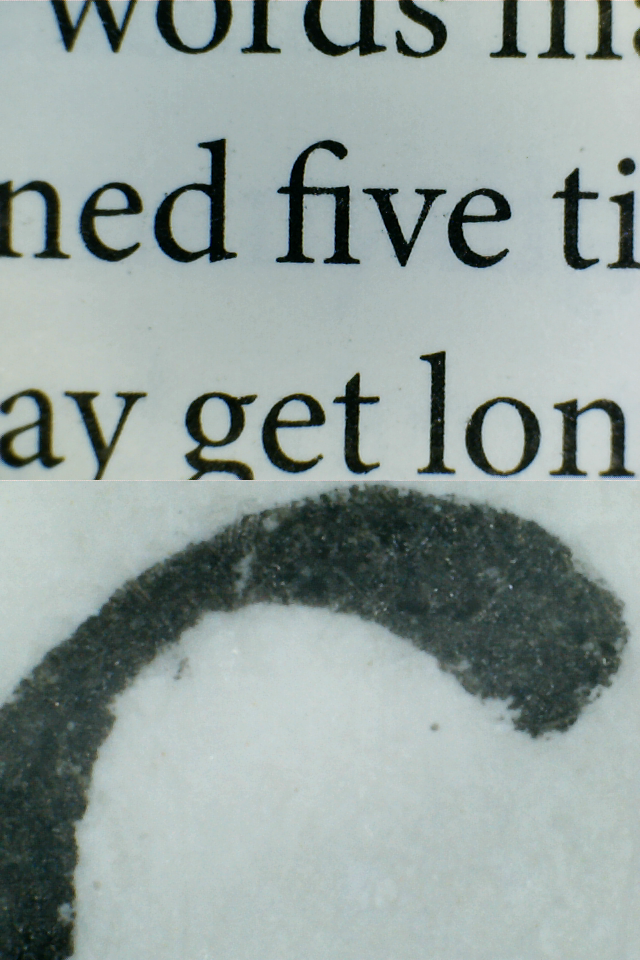
\includegraphics[width=0.31\textwidth]{gfx/sc-book}\label{fig:scr:print}} \hspace{1mm} 
        \subfloat[][A laser-printed webpage]{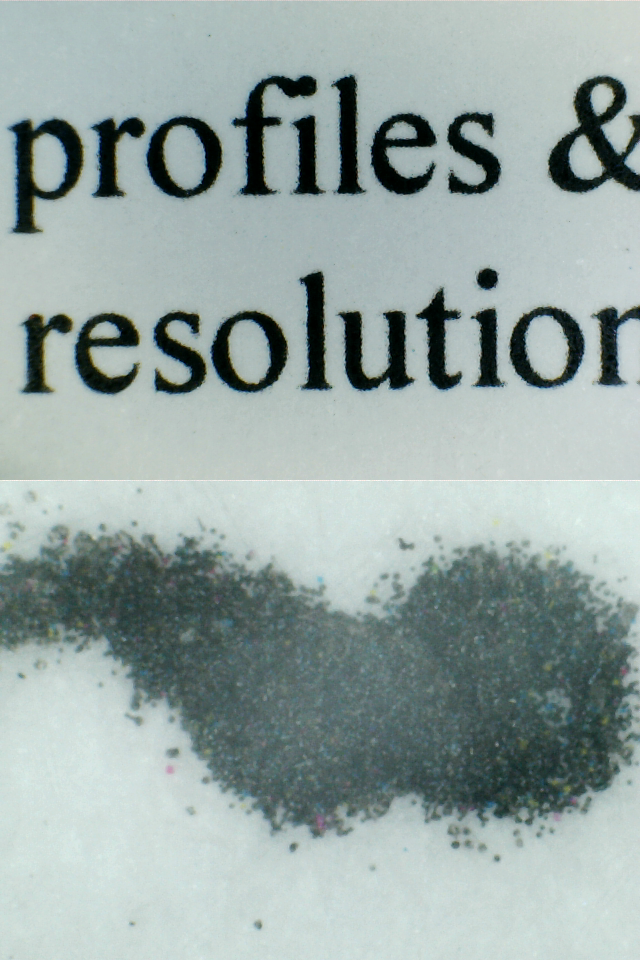
\includegraphics[width=0.31\textwidth]{gfx/sc-laser}\label{fig:scr:laser}} \hspace{1mm} 
        \subfloat[][A dot-matrix \textsc{lcd} screen]{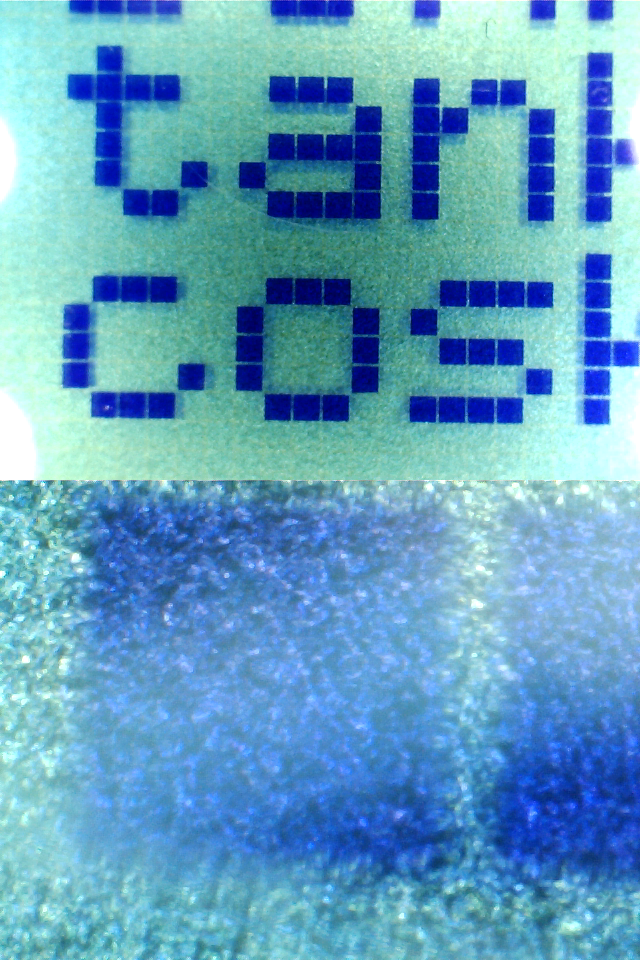
\includegraphics[width=0.31\textwidth]{gfx/sc-lcd}\label{fig:scr:calculator}} 

        \subfloat[][A \textsc{tft} \textsc{lcd} monitor]{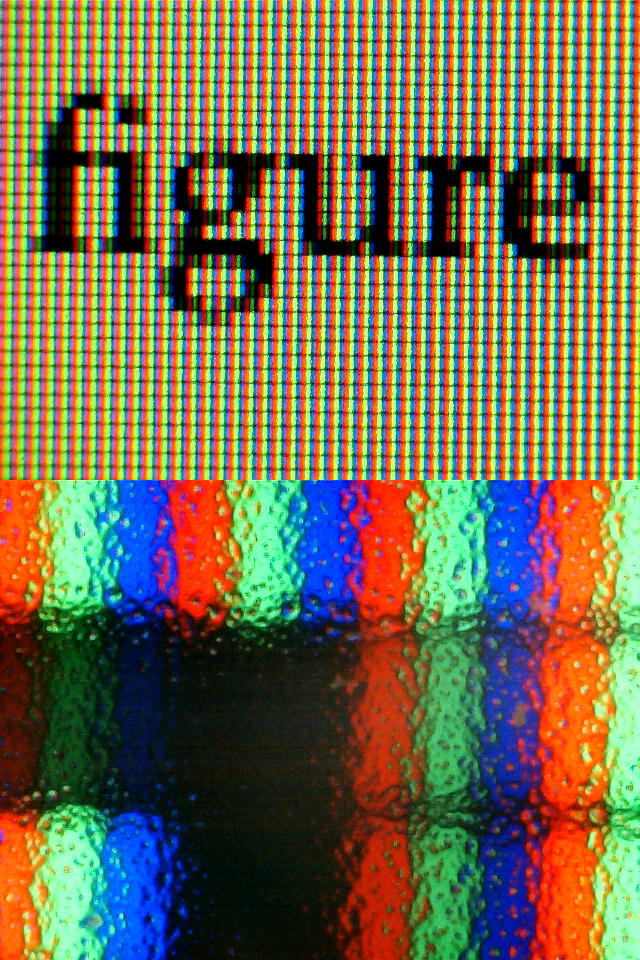
\includegraphics[width=0.31\textwidth]{gfx/sc-tft1}} \hspace{1mm} 
        \subfloat[][Another \textsc{tft} \textsc{lcd} monitor]{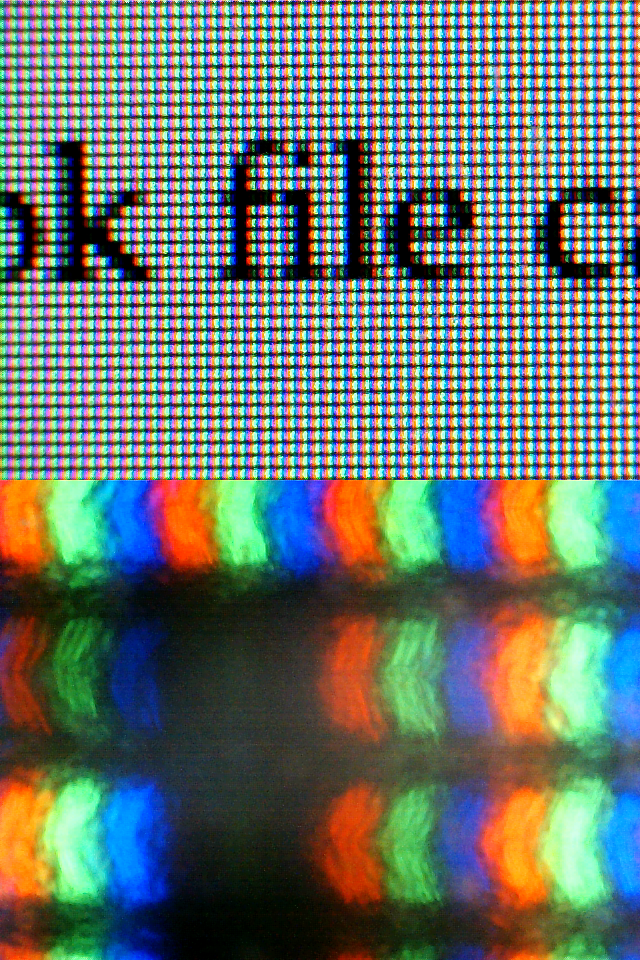
\includegraphics[width=0.31\textwidth]{gfx/sc-tft2}} \hspace{1mm} 
        \subfloat[][A \textsc{tft} \textsc{lcd} on a Kindle Fire HD]{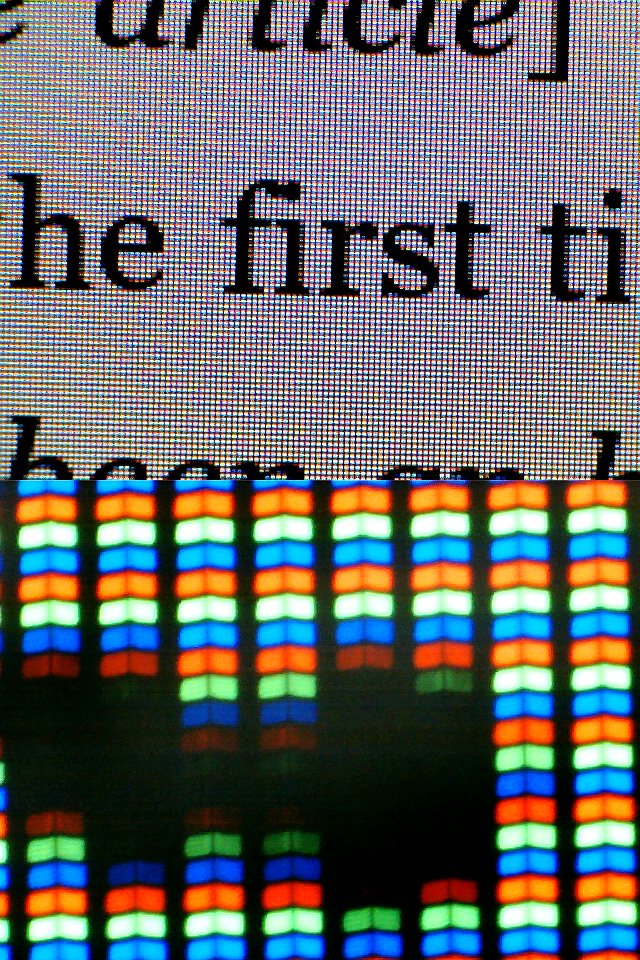
\includegraphics[width=0.31\textwidth]{gfx/sc-fire}} 

        \subfloat[][A Super \textsc{amoled} display on a Galaxy Nexus smartphone]{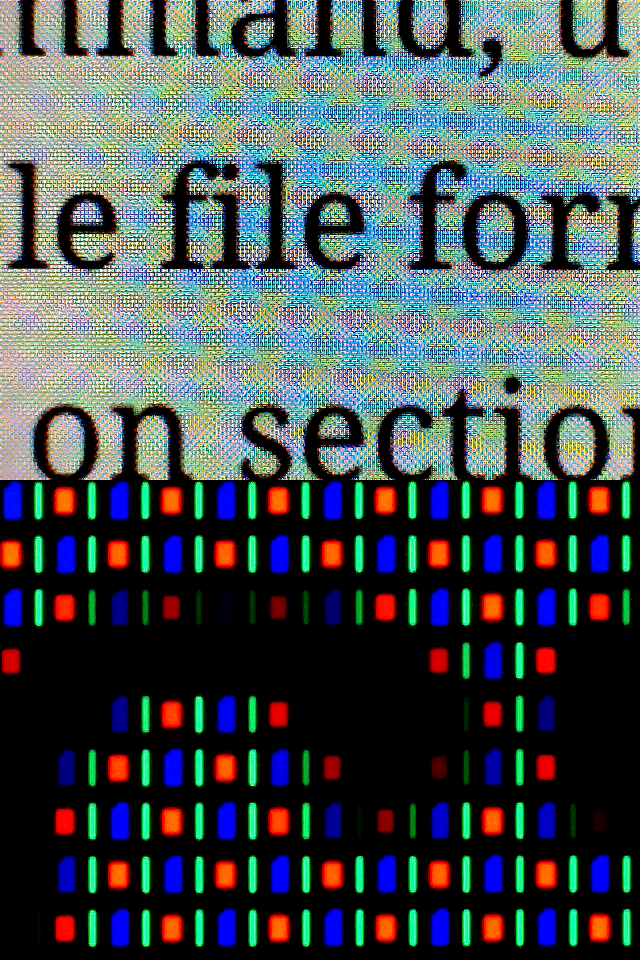
\includegraphics[width=0.31\textwidth]{gfx/sc-gnex}} \hspace{1mm} 
        \subfloat[][An electronic paper display on a Kobo eReader]{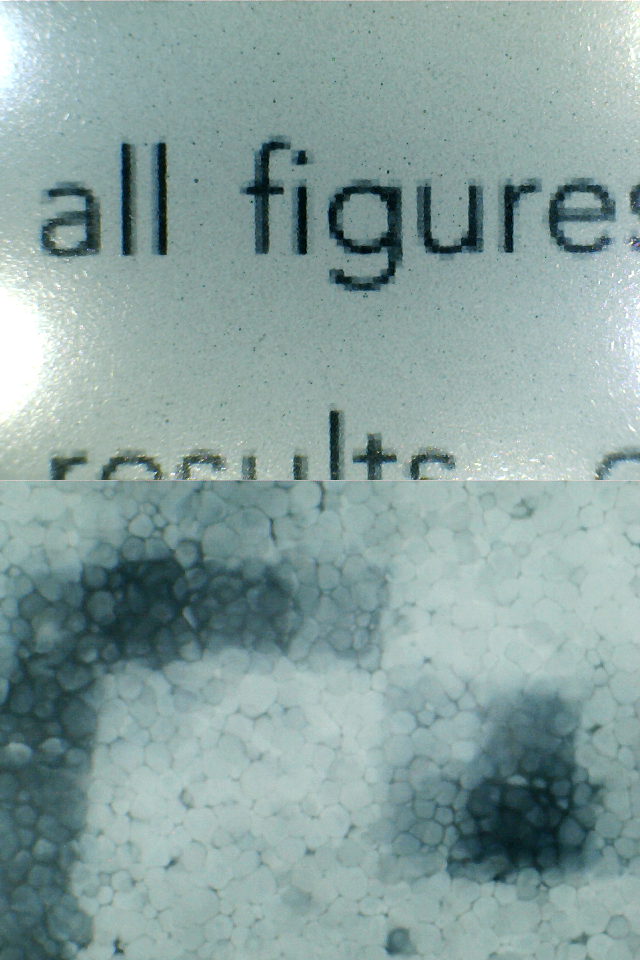
\includegraphics[width=0.31\textwidth]{gfx/sc-kobo}\label{fig:scr:kobo}} \hspace{1mm} 
        \subfloat[][An electronic paper display on a Kindle Touch]{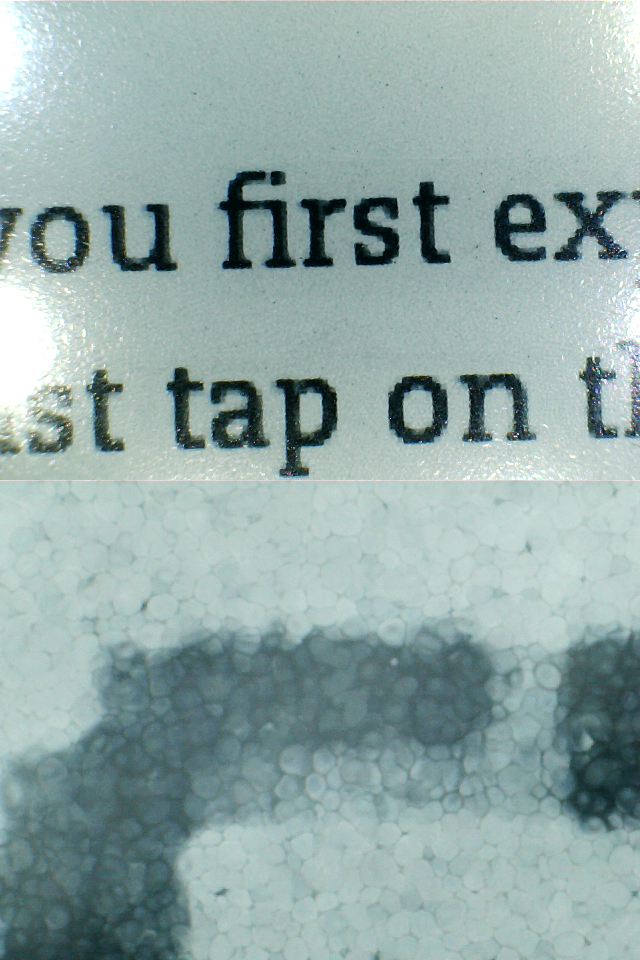
\includegraphics[width=0.31\textwidth]{gfx/sc-kindle}\label{fig:scr:kindle}} 

    \end{centering}

    \caption[Examples of document display technologies]{Examples of some document display technologies, magnified about 25 times (top halves of images) and 350 times (bottom halves). Note that the resolutions of the screens in (f) and (g) are close to that of the microscope used to capture the image, hence the aliasing effect.}
    \label{fig:screens}
\end{figure}


\section{``Good'' typesetting}
\label{sec:goodtypesetting}

Generally speaking, the better the quality of a document's typography, the less it should be noticed by the reader. Good typography should be transparent, in order that the reader may concentrate upon the content of the document, rather than be distracted by its presentation.

Many studies~\cite{Mittelbach1992,Hill1999,Bringhurst2008,Voorhees2011,Legge2011} have confirmed that the readability of text is inextricably linked to the quality of its typography. In particular, it is stated in \emph{The Magic of Reading}~\cite{Hill1999} that both regularity of whitespace between words and the evenness of line lengths are of importance\ed the only way to achieve this is to use a line-breaking algorithm that attempts to make line lengths as even as possible. Unfortunately, producing well-typeset text can be an extremely complex process.


\subsection{Hyphenation and Line-Breaking}
\Ebook{} readers typically use a ``greedy'' algorithm to lay out their text\ed that is, they place as many words as will fit onto the current line without exceeding it, then start a new line and continue. Although this algorithm is optimal in that it will always fit text onto the fewest possible lines, it often causes consecutive lines to have wildly varying lengths, accentuating either the ``ragged-right'' effect of the text, or, in the case of justified text, the inter-word spacing. In general, \ebook{} readers will only hyphenate in extreme cases\ed indeed the Kindle seems not to do so at all, to the detriment of its typography (see Figure~\ref{fig:crapkindle}).

\begin{figure}
    \centering
    \fbox{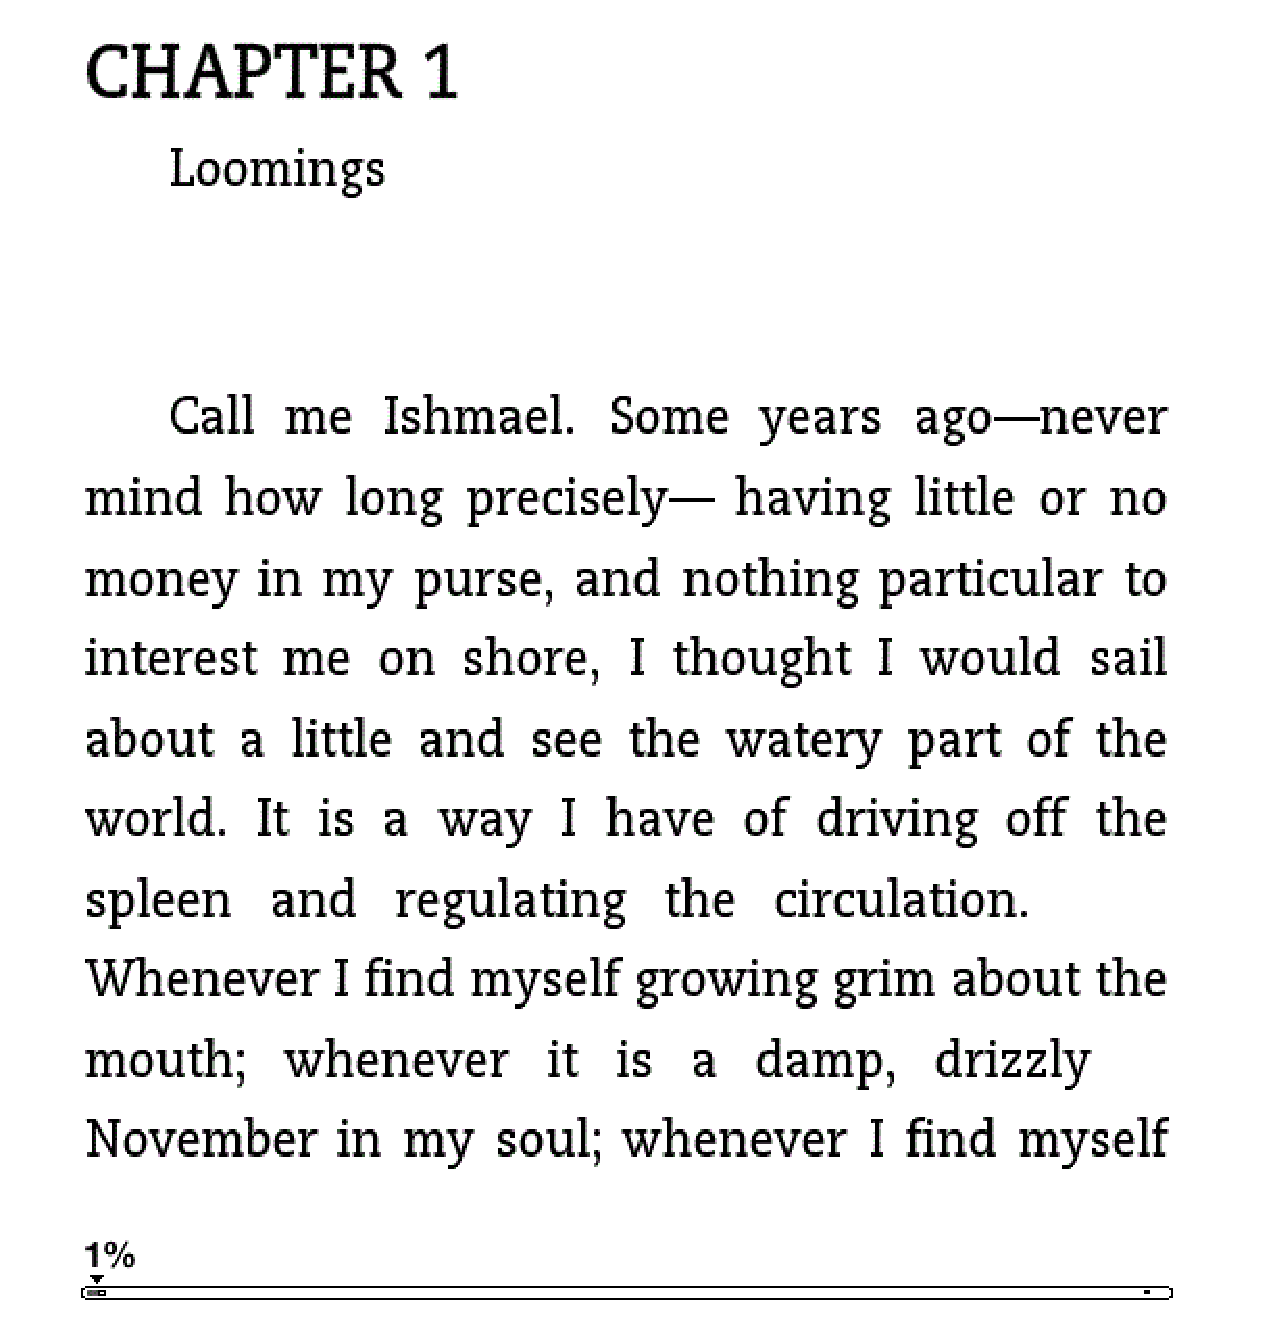
\includegraphics[width=\textwidth
]{gfx/screen_shot-42583}}
    \caption[Poor typography on the Kindle]{The Kindle appears to fully justify its text, falling back to ragged-right when inter-word spacing would become too large. Its lack of a hyphenation algorithm exacerbates this problem.}
    \label{fig:crapkindle}
\end{figure}

Donald E. Knuth and Michael F. Plass~\cite{Knuth1981} developed a more advanced line-breaking algorithm (now used by \TeX{}) which attempts to minimise large discrepancies between consecutive lines by considering each paragraph as a whole. \TeX{} also uses the hyphenation algorithm designed by Franklin Liang~\cite{Liang1983} (another of Knuth's grad students) which has been ported to many other applications. Figure~\ref{fig:greek} compares the Knuth-Plass algorithm against the default layout of a web browser (a first fit, greedy approach).


\begin{figure}
\begin{center}
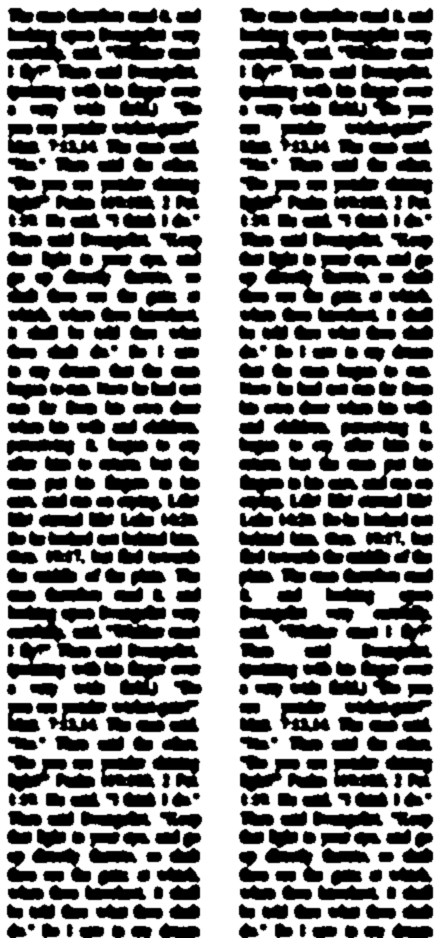
\includegraphics[height=0.8\textheight]{gfx/greek}
\end{center}
\caption[Knuth-Plass layout versus a first-fit algorithm]{Knuth-Plass layout (left) versus a first-fit algorithm (right). The text has been greeked to draw attention to layout rather than content. Note that Knuth-Plass results in looser spacing of certain lines where it helps avoid extremely loosely-set lines ahead. Even without using hyphenation (this implementation of Knuth-Plass does not include a hyphenation algorithm) the differences are noticeable. }
\label{fig:greek}
\end{figure}

Knuth and Plass's line breaking algorithm, in conjunction with Liang's hyphenation algorithm, breaks paragraphs into lines of text to fit a page, resulting in what can be considered an aesthetically optimal configuration. \TeX 's default behaviour is then to alter the spacing between words in order to justify the line to fit the measure of the page. This algorithm nominally runs in $O(n^2)$ time (compared with $O(n)$ for a greedy first-fit approach), although with some pruning, the effective complexity can be reduced to nearer $O(n)$.~\cite{Hirschberg1987,Eppstein1992,Hurst2009} In practice though, large constant factors still make the algorithm slow. In any case, the Knuth-Plass algorithm is certainly not the last word in line-breaking algorithms: for example, it has no mechanism to avoid (nor indeed any knowledge of) vertical rivers of whitespace.~\cite{Mittelbach1992} Inevitably, adding support to avoid rivers, and for any of the other nuances used by hand compositors, would add further complexity.



\begin{figure}
 \fbox{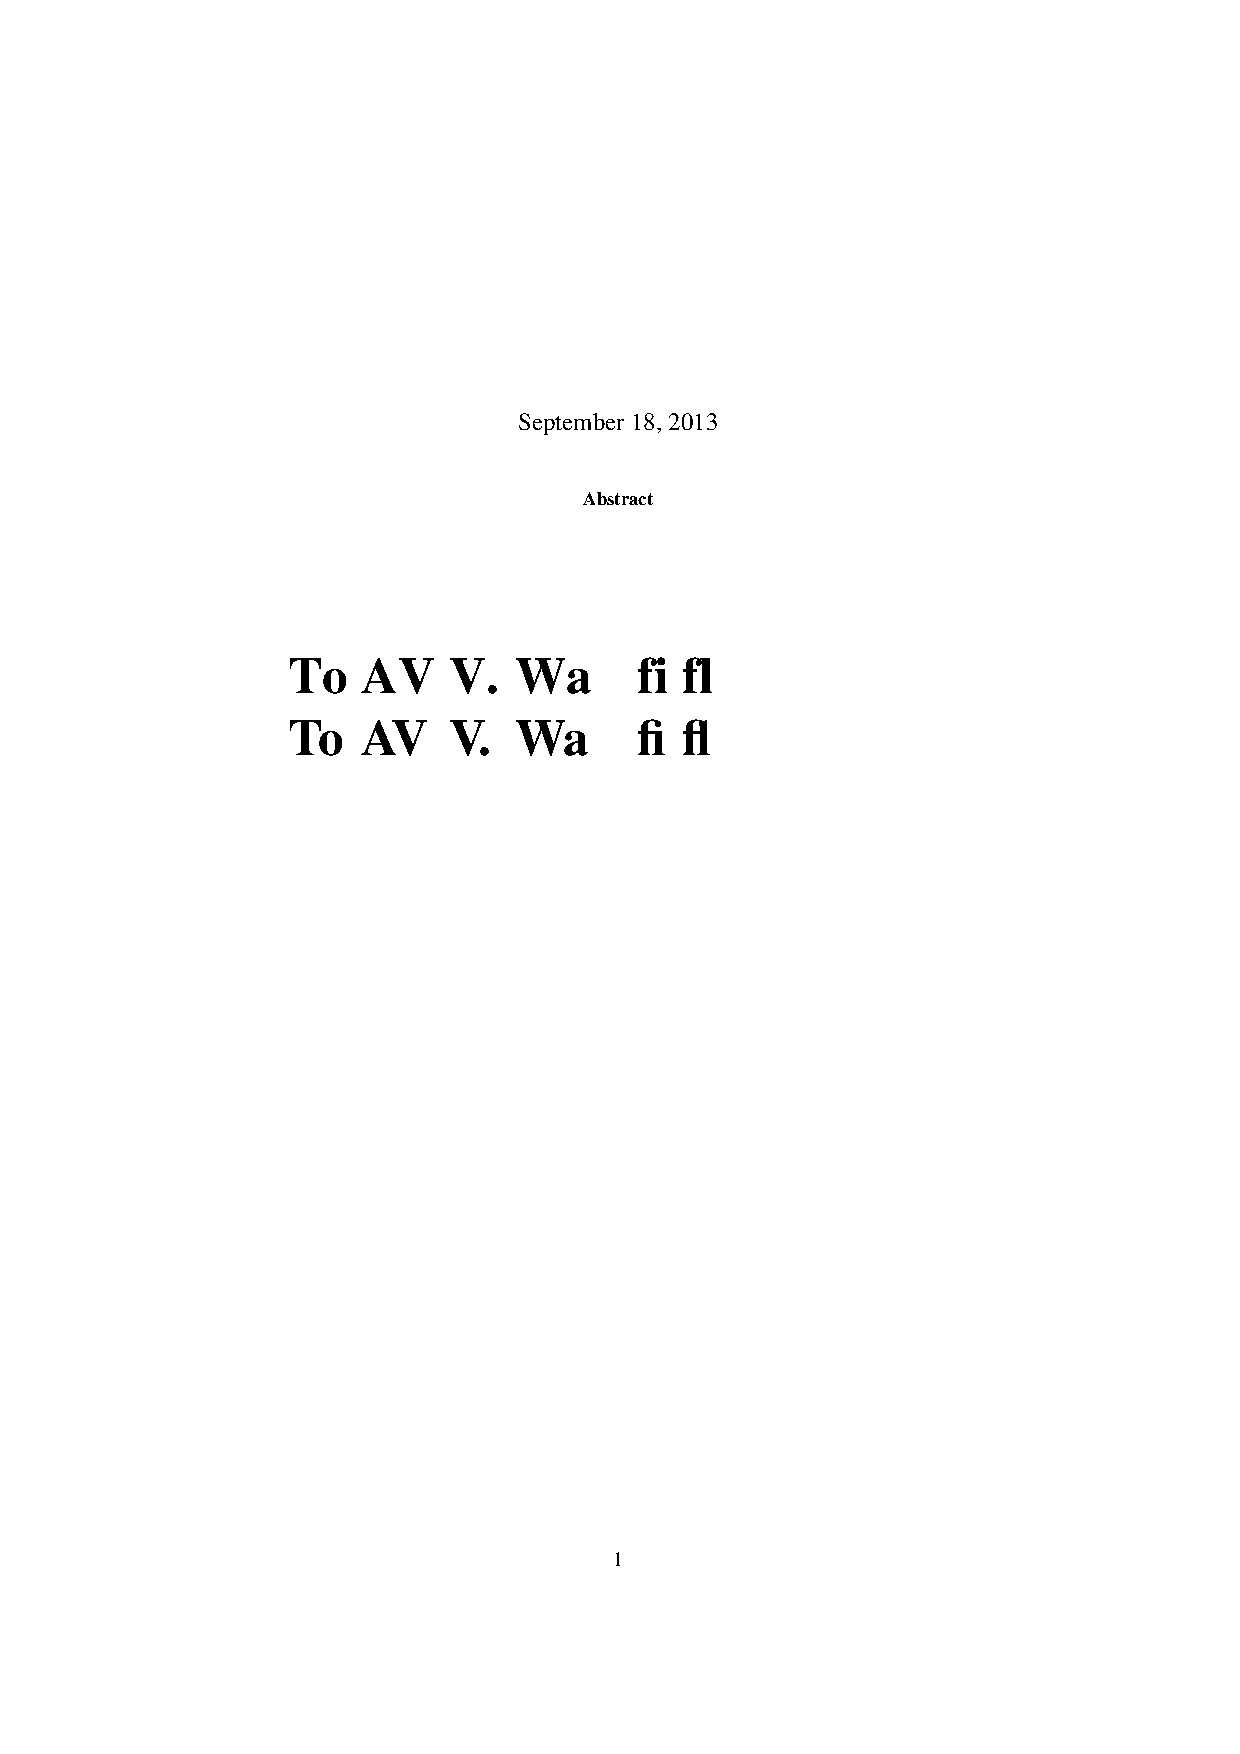
\includegraphics[trim=1.8in 6.54in 3.4in 4.25in, clip=true, width=\textwidth]{gfx/kerningetc}}
 \caption[Examples of microtypographical techniques]{Examples of various letter-pairs and their kerned (left) or ligature (right) equivalents, as typeset by pdf\LaTeX{}. Some further examples of fi ligatures (or not) can be seen in Figure~\ref{fig:screens}.}
 \label{fig:kern-lig}
\end{figure}


\subsection{Microtypographical Techniques}
\label{sec:microtypography}
Other techniques employed during hand-type\-set\-t\-ing, and high-qua\-l\-ity electronic typesetting, include the use of what is often termed \emph{micro\-typo\-graphy},~\cite{Hurst2009} such as the use of kerning and ligatures. Kerning involves altering the spacing between certain glyph pairs in order to give the appearance of more consistent letter spacing, and ligatures are sin\-gle-glyph replacements for two or more single glyphs that may otherwise have had clashing components. Some examples of these are shown in Figure~\ref{fig:kern-lig}.

Kerning requires a table of kern-pairs, specific to each font; values from this table must then be looked up for every pair of adjacent glyphs in the document. Ligatures may or may not need to be inserted: if the component characters of the ligature lie over a potential hyphenation point, it cannot be decided whether to replace them with the ligature until it is known whether the hyphenation point needs to be used. \TeX{} handles kerning and insertion of ligatures automatically, but there are still further typographical tweaks that its default typesetting algorithm does not use.

More\marginpar{\emph{pdf\LaTeX}, used to typeset this thesis, \emph{does} tweak tracking and glyph widths when justifying text} advanced methods than simply stretching or shrinking the word spacing do exist, however. Robert Bringhurst, in \emph{The Elements of Typographic Style},~\cite{Bringhurst2008} suggests that in addition to altering word spacing, subtle changes to inter-character spacing (also known as \gls{tracking}) and to individual glyph widths (in the range of $\pm$ 3\%) can produce more typographically and aesthetically pleasing results.




\section{Paradigms of Document Representation}
Computer representations of documents can be classified into two distinct paradigms:
\begin{itemize}
 \item Documents stored in \emph{fixed formats}, such as \pdf{} and PostScript, are designed to be the direct analogues of printed pages
 \item Documents stored in \emph{flowable formats}, such as the \html{}, have no fixed presentation associated with them, thus their layouts must be computed each time the documents are displayed
\end{itemize}
Currently there is no middle ground\ed a document may either be fully rendered to a fixed layout, or completely unrendered, to be laid out at the mercy of a display device's decisions.

\subsection{Fixed Formats}
\label{sec:fixedformats}
The only fixed document format commonly used for \ebook{}s (or indeed commonly used at all) is \pdf{}, which was originally designed as a way of faithfully reproducing documents both on screen and in print.~\cite{Warnock1991} For this reason, it is almost entirely pre\-s\-en\-ta\-tion-oriented and will not necessarily include any metadata pertaining to the semantic structure of a given document.

The archetypal \pdf{} file consists solely of drawing operators which describe the document pages. There is no compulsion for these drawing operators to render the page in an order that might be considered sensible by a human reader. For example, if a \pdf{} generator program decided to render every character on a page in alphabetical order, or radially outwards from the centre, the resulting file would still be semantically valid, and the result would be imperceptible to the reader.

This lack of imposed semantic structure makes it difficult to infer the best way to ``unpick'' \pdf{} files to allow their content to be reflowed into a new layout. For example, it is not easy to decide programatically whether a line break between adjacent lines of text is explicitly intended to be there (for example, the end of a paragraph) or if it is an artefact of the document layout. As an example, the Adobe Reader app for Android cheerfully offers to reflow \pdf{} pages should you require it, but usually results in what can be seen in Figure~\ref{fig:acrobatreflow}.

\begin{figure}
\fbox{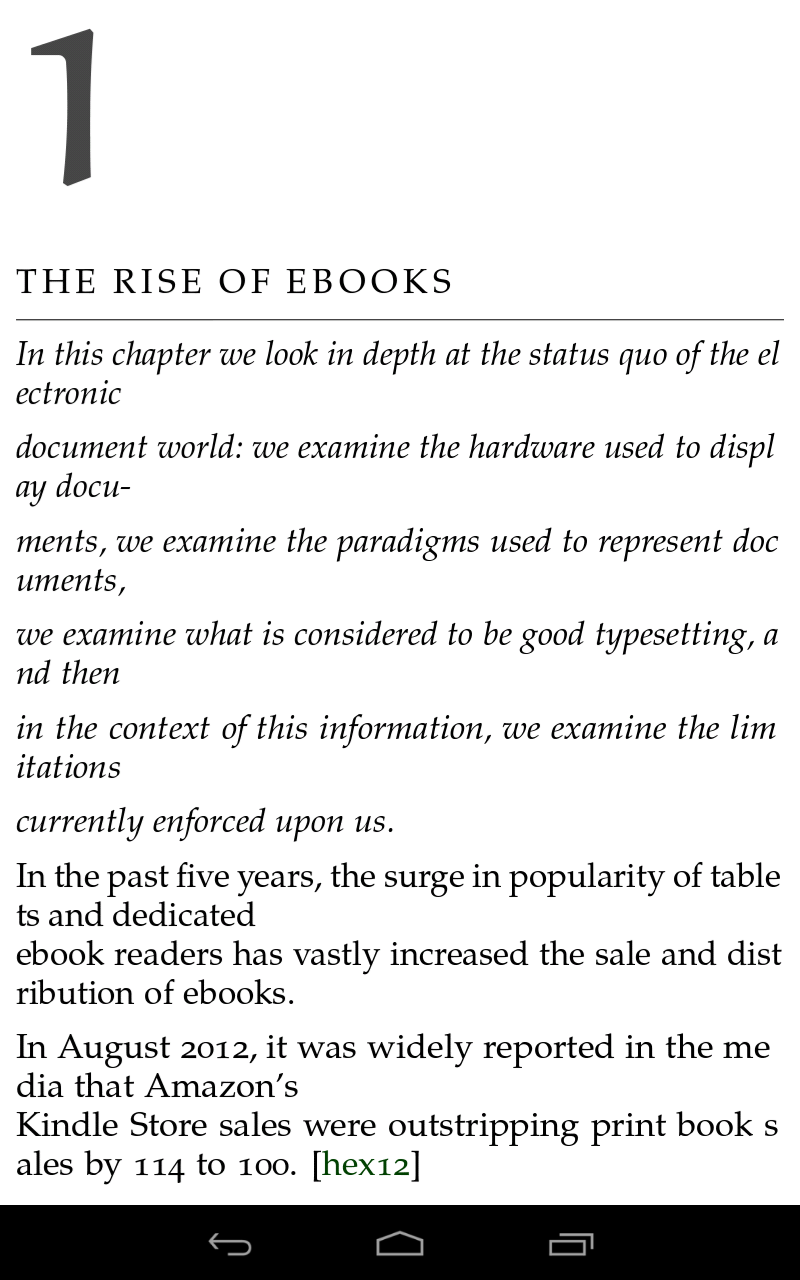
\includegraphics[width=\textwidth]{gfx/acrobatreflow}}
\caption[Reflowed text of a \textsc{pdf} file]{Adobe's Reader app for Android includes an option that allows \pdf{} files to be reflowed, but the lack of semantic structure within most \pdf{} files limits the process to using only what can be inferred from the original layout. This figure shows the start of this chapter reflowed by the app.}
\label{fig:acrobatreflow}
\end{figure}

It would be inaccurate to state that \pdf{} files \emph{cannot} represent the semantic structure of their content\ed indeed as early as 1999, \pdf{}~1.3 introduced \emph{logical structure} facilities,~\cite{Adobe2001} adding an optional \emph{structure tree} to the \pdf{} specification, and \emph{tagged \pdf{}}, introduced in \pdf{}~1.4 in 2001, provides various extensions to this. \pdf{} documents which actually make good use of these facilities are few and far between, even a decade after their introduction.

%Unfortunately, even when these facilities to include structural semantics are actually used, it is still not particularly useful in reflowing the content of documents. It is true that it helps to correctly identify the logical order of page components, but 

%If a document is stored at a higher, more abstract level than \pdf{}, the text can be rendered at any desired size, at the cost of the retention of high-quality typesetting afforded by \pdf{}.

\subsection{Flowable Formats}
\label{sec:flowableformats}

The\marginpar{Amazon's proprietary Kindle format is derived from Mobipocket; \pdf{} and \epub{} are open standards} two most common flowable \ebook{} formats are \epub{} and Mobipocket, both of which are largely based on \html{}. \html{} was chosen not only because of its inherent support for reflow, but also because it allows document content to be semantically marked up into paragraphs, various levels of headers, and so on. At the time, this was an enormous improvement over \ebook{}s stored as plain text, which consequently had neither formatting nor semantic structure. 

Whilst the use of these \html{}-like formats allows the semantic structure of documents to be very well defined, in general their presentation can only be specified in a very loose manner. On an \ebook{} reader (or in \ebook{} reading software) the user is often presented with a choice of typefaces and point sizes, which gives the e-reader software some scope for rendering the document in arbitrary ways.

Since a document stored in a flowable format has no concrete presentation associated with it, each time the document is displayed, its layout must be recomputed. For an \ebook{} reader to maximise its battery life, this computation must be as simple as possible. As a consequence, the algorithm used must not be too complex, since the more \textsc{cpu} cycles spent executing it, the less time the \textsc{cpu} can spend idle, and thus the greater the drain on the device's battery.


\section{Limitations of Current Formats}

The design paradigm of \pdf{}, conceived in the early 1990s,~\cite{Warnock1991} was to form a perfect analogue of the printed page, which would be exactly reproducible regardless of the system on which the file was rendered. For this reason, it is possible to embed fonts within \pdf{} files, to ensure faithful reproduction on any system, regardless of which fonts are actually installed. In general, a well typeset \pdf{} file looks good wherever it is displayed, but, stemming from the ``digital sheet of paper'' paradigm, page sizes in a \pdf{} document are necessarily fixed at creation-time. An overwhelming majority of \pdf{} documents are rendered for  \textsc{us} letter or \textsc{a}4 size paper. This is fine if the document is to be printed and read. On a reasonably large screen, the document remains perfectly readable, and on a 10'' netbook or tablet screen it may provide an acceptable reading experience. Anything much smaller (notably mobile phones, and \ebook{} readers) requires a combination of zooming and panning  in order to read the document.

Documents may, of course, be rendered to a smaller page size, but the problem still remains\ed it is unlikely that any one page size will be suited to \emph{all} reading platforms. Most \ebook{} readers, using their native (i.e.\ non-\pdf{}) formats, allow text to be resized according to user preference. Indeed, it seems unnecessarily restrictive to force one size of type upon the user. Of course, while physical books suffer from this affliction, \ebook{}s need not. Selling \ebook{}s separately in standard and large-print versions seems perverse when, for virtually no difference in cost to the publisher/distributor, both can be included in one file.

Systems to reflow the content of PDF documents have been devised,~\cite{Lovegrove1995,Marinai2013} but as noted in Section~\ref{sec:fixedformats}, this is often extremely difficult to accomplish satisfactorily. Even when the logical order of page components can be identified correctly, the benefit of any precomputed high-quality typesetting is lost if the text itself must be re-typeset.



\epub{} and Mobipocket, both based on \html{}, provide a higher level of abstraction for documents, whereby the logical structure of their content is still present. They allow many rendering decisions to be made at view-time, such as choice of typeface and font size. Line breaks and page breaks are then calculated and inserted as necessary, in order to wrap the text to fit the screen, and to paginate the content.

The rendering engines of \ebook{} readers use simplistic reflow algorithms\ed but necessarily so. One of the major bottlenecks in today's portable electronic devices is their battery life: battery capacity has not improved at anywhere near the same rate as other facets of mobile computing. Manufacturers of \ebook{} readers may claim their products have batteries that can last for weeks, but this is principally due to the many typographical corners that they cut when laying out flowable content. As noted in Section~\ref{sec:flowableformats}, were these devices to use more complex layout algorithms, which can produce far higher quality typeset output, any savings made by using a low-power electronic paper screen would quickly be lost. Furthermore, the more time that is spent formatting the output, the longer the delay between page turns on the device, given that each subsequent page is only rendered when a page turn is requested. This time delay could be shortened by precomputing the layout of subsequent pages between page turns, but this would not solve the battery-drain problem.


\epub{} allows fonts to be embedded, but Mobipocket does not. Mobipocket files (and by extension, Kindle files)\marginpar{Amazon has begun to address this issue by developing a new format, \textsc{kf8}, still Mobipocket-based, that allows more complex styling,\\ in a manner comparable to \textsc{epub}} are therefore restricted to be rendered in a typeface local to (and often chosen by) the reader software. The Kindle, as an example, provides the user with a choice of ``regular'', ``condensed'', or ``sans-serif'' for the main body text of its documents. There are bold and italic variants of these, which are applied according to formatting instructions within the documents themselves. Additionally, there is a typewriter-style font which document authors may choose to use in the same manner.

\begin{figure}
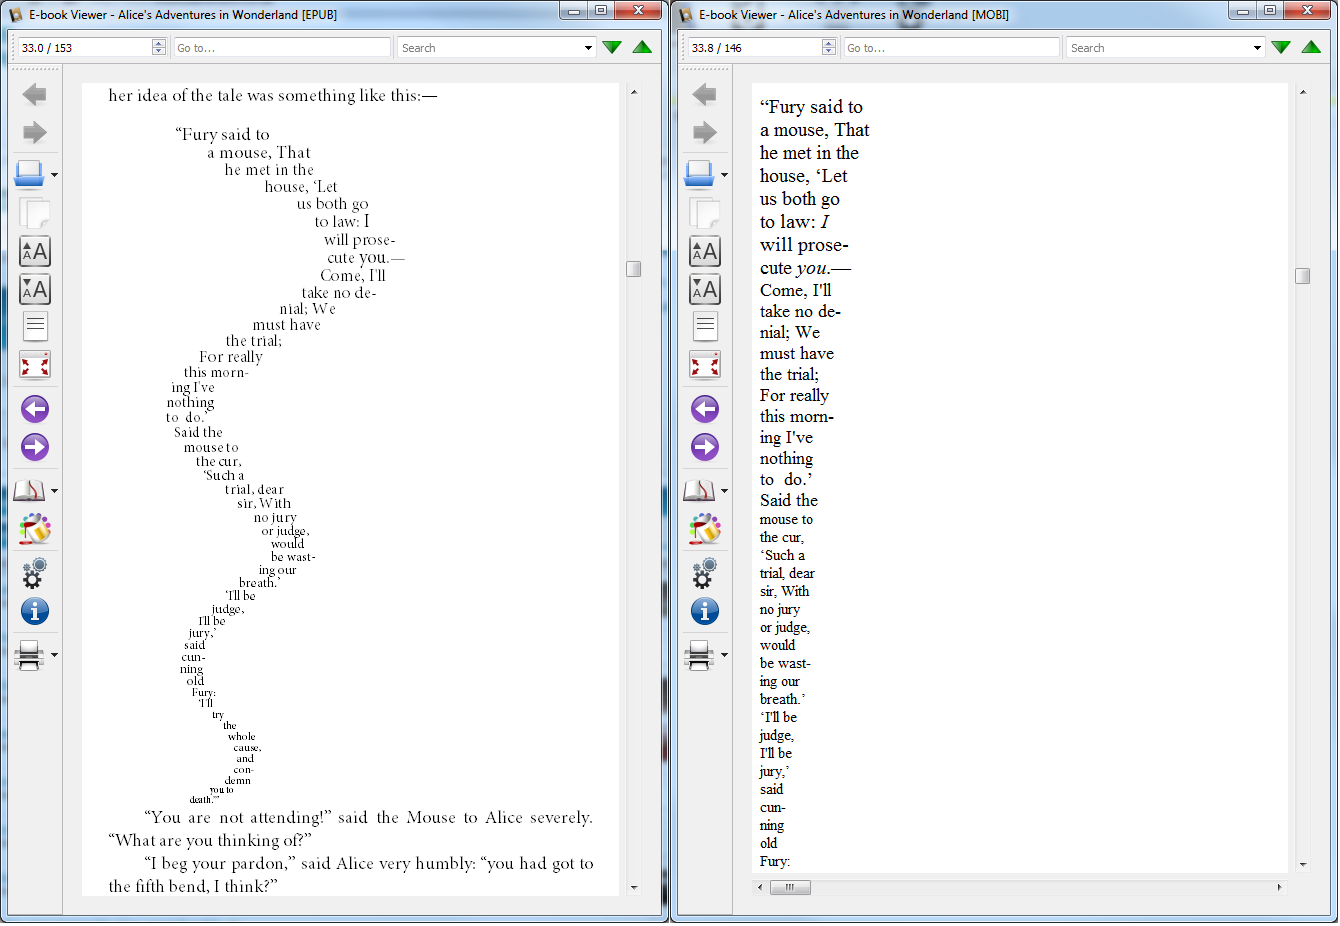
\includegraphics[width=\textwidth]{gfx/alices1}
\caption[Document displayed in Calibre]{On the left is an \epub{} version of Alice in Wonderland, displayed in Calibre (an open source desktop \ebook{} viewer). On the right is the same file, converted to Mobipocket, also displayed in Calibre. Note that in addition to the indentation being lost, the (embedded) font from the \epub{} is no longer present in the Mobipocket file.}
\label{fig:alices1}
\end{figure}



The Mobipocket specification supports a very limited subset of \html{} and \css{}, which makes it virtually impossible to achieve complex layouts such as those involving arbitrary indentation or font size changes. Figures \ref{fig:alices1} and~\ref{fig:alices2} demonstrate the well known ``Mouse's Tale'' from Lewis Carroll's \emph{Alice in Wonderland}, and the limitations of various formats.


\epub{} is a little more flexible, since it supports a more comprehensive range of \xhtml{} and \css{}, has support for \textsc{svg}, and allows for arbitrarily complex styling. \epub{} files are still entirely reliant on the rendering engine of the display device correctly displaying their content, as they have no concrete layout associated with them.





\section{Summary}

We have so far seen that electronic representations of documents have layouts that are either fully fixed, or fully flowable. Currently there is no middle ground. Documents with fixed layouts may be of arbitrarily high typographic quality, since their layout is fully computed when they are created. Documents with flowable layouts are not provided with any guarantee that their content will be laid out with any semblance of typographic quality. In any case, to compute a high-quality layout in real-time is difficult, especially on a low-powered portable device such as an \ebook{} reader.

\begin{figure}
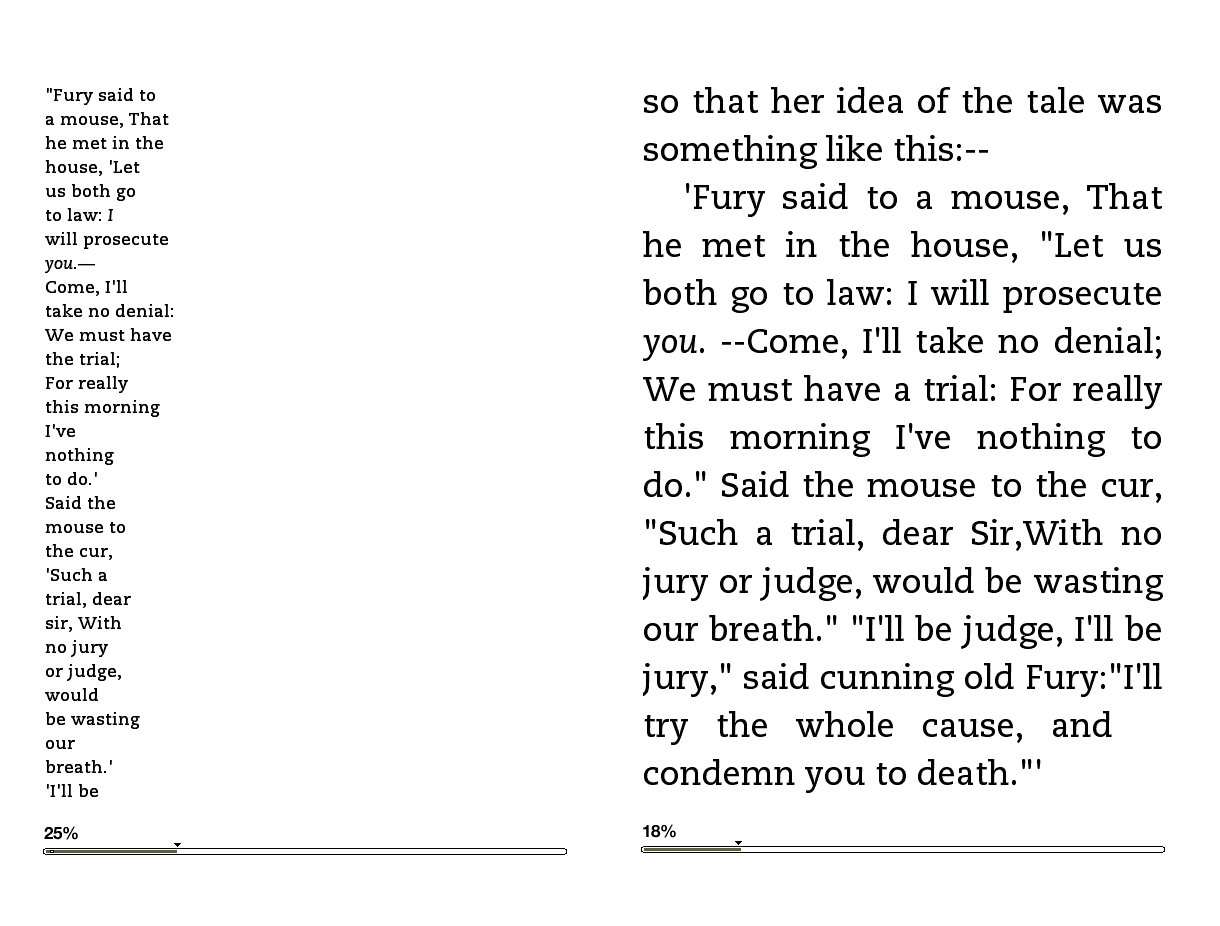
\includegraphics[width=\textwidth]{gfx/alices2}
\vspace{-0.2in}
\caption[Same document displayed on the Kindle]{On the left is the Mobipocket version of Alice in Wonderland (from Figure~\ref{fig:alices1}) displayed on the Kindle. Note that the sizing instructions appear to have been ignored. On the right is the free version of Alice in Wonderland from the Kindle store, displayed on the Kindle. Note that no attempt has been made to render the poem in a ``tail'' shape.}
\label{fig:alices2}
\end{figure}

We have seen that screen technologies for \ebook{} readers have been evolving to become better and better, allowing documents to be displayed in a quality that rivals physical, printed pages. Document representation paradigms have not caught up. They are based on technologies that have been repurposed to be used in ways they were never designed. Fixed layout representations were designed for display on paper. Flowable layout representations were designed for display on such low-resolution screens (\eg{} that in Figure~\ref{fig:scr:calculator}) and underpowered devices that quality typography would have been nothing but a pipe dream.


\section{Contributions of this Thesis}

It is clearly time for a new document representation paradigm to be devised, in order to catch up with contemporary document display technologies\ed it is time for the introduction of a more \emph{malleable} document format. There has been little research into this area in the past. Much effort has been put into high-quality typesetting for documents with fixed layouts. Much effort has been put into providing styling for documents with flowable layouts\ed notably via css\ed but virtually no consideration has been given to producing well-typeset output on the fly, particularly with the minimum required computation.

In this thesis, such a novel document representation paradigm, geared towards use on portable devices, is proposed and implemented. The desired malleability is afforded to documents by precomputing key parts of the typesetting process, which allows their content to be gently coaxed to fit any page size, without compromising the quality of their typography.



\section{Thesis Structure}

This introductory chapter is designed to provide an overview of the present state of affairs of the electronic document world, with particular emphasis upon the technologies used in contemporary \ebook{} readers. 

Chapter~\ref{ch:malleable} describes the first prototype implementation of a system to generate and display simple malleable documents.

Chapter~\ref{ch:floats} describes a complete reimplementation of the system described in Chapter~\ref{ch:malleable}, and extends the devised model to include support for floating items such as figures and tables.

Chapter~\ref{ch:bloat} addresses the issue of enlarged file sizes, and details various methods to keep file sizes to a minimum.

Chapters \ref{ch:techanalysis} and~\ref{ch:aesthetics} provide technical and aesthetic analysis, focusing on the quantitative and qualitative aspects of the system as it runs at view-time.

Finally, Chapter~\ref{ch:conclusions} evaluates the success of the project, and details areas of potential new research that have been encountered throughout the process.
